% =====================================================================
%  Capítulo 7 — Resolução numérica
%  Inserir antes da seção de exercícios.
% =====================================================================
\section{Resolução numérica}
\label{sec:cap07-numerica}

Este capítulo afirmou três coisas que só ficam realmente convincentes quando
viram número: que a conexão pode ser não nula sem haver curvatura, que o
tensor de Riemann é a rotação produzida por um circuito fechado, e que a
curvatura controla a aceleração relativa de geodésicas vizinhas. Aqui as três
são medidas. E, de quebra, montamos uma máquina que extrai $\Gamma$, Riemann,
Ricci e Kretschmann de uma métrica qualquer, por diferenças finitas --- a
mesma que será apontada para Schwarzschild nos capítulos seguintes.

\subsection{Python}

\programa[Transporte paralelo e holonomia, tensor de Riemann por diferenças finitas e desvio geodésico. Contém a máquina genérica que calcula $\Gamma$, Riemann, Ricci e Kretschmann de qualquer métrica.]{codigo/cap07\_curvatura.py}

\subsubsection*{Transporte paralelo e holonomia}

Transportar um vetor ao longo de uma curva significa resolver
\begin{equation}
  \rd{V^a}{\lambda}
  = -\Gamma^a{}_{bc}\,V^b\,\rd{x^c}{\lambda},
  \label{eq:cap07-transporte}
\end{equation}
que é uma equação diferencial ordinária comum. Se o circuito é fechado, o
vetor volta ao ponto de partida --- e a pergunta é se ele volta igual a si
mesmo. O ângulo de discrepância é a \emph{holonomia}.

\begin{atencao}
O ângulo tem de ser medido em relação a uma direção \emph{fixa}, não em
relação à base coordenada --- que ela própria dá uma volta completa ao
percorrer o circuito. Esquecer esses $2\pi$ é o erro que faz a holonomia da
esfera dar o valor errado justamente para as calotas maiores que um
hemisfério. No código, o acerto é uma linha: acumular o ângulo com
\texttt{np.unwrap} e somar $2\pi$ no fim.
\end{atencao}

\begin{saida}
\begin{lstlisting}[style=rgsaida]
plano euclidiano em coordenadas polares (Christoffel nao nulos):
   circuito r =  0.5:  holonomia = +1.087e-11 rad
   circuito r =  1.0:  holonomia = -6.566e-12 rad
   circuito r =  2.0:  holonomia = -4.145e-11 rad
   circuito r =  4.0:  holonomia = +1.678e-10 rad
esfera unitaria (a holonomia deve ser a area da calota):
   theta_0     holonomia   area 2pi(1-cos)        erro
    0.5000    0.76917145        0.76917145    3.89e-10
    1.0000    2.88836580        2.88836580    2.25e-10
    1.5708    6.28318531        6.28318531    8.88e-16
    2.0000    8.89791300        8.89791300    1.62e-10
    2.6000   11.66717613       11.66717613    3.38e-10
\end{lstlisting}
\end{saida}

\begin{central}
As duas metades desta saída são a tese do capítulo. No plano em coordenadas
polares, $\Gamma^r{}_{\phi\phi}=-r$ e $\Gamma^\phi{}_{r\phi}=1/r$ são não
nulos, o integrador trabalha de verdade --- e o vetor volta \emph{exatamente}
como saiu, a $10^{-11}$. Na esfera, a holonomia coincide com a área
envolvida em oito casas decimais. Conexão é artefato de carta; holonomia é
geometria. Este é o conteúdo operacional da frase ``Christoffel não é
curvatura''.
\end{central}

\begin{figure}[htbp]
  \centering
  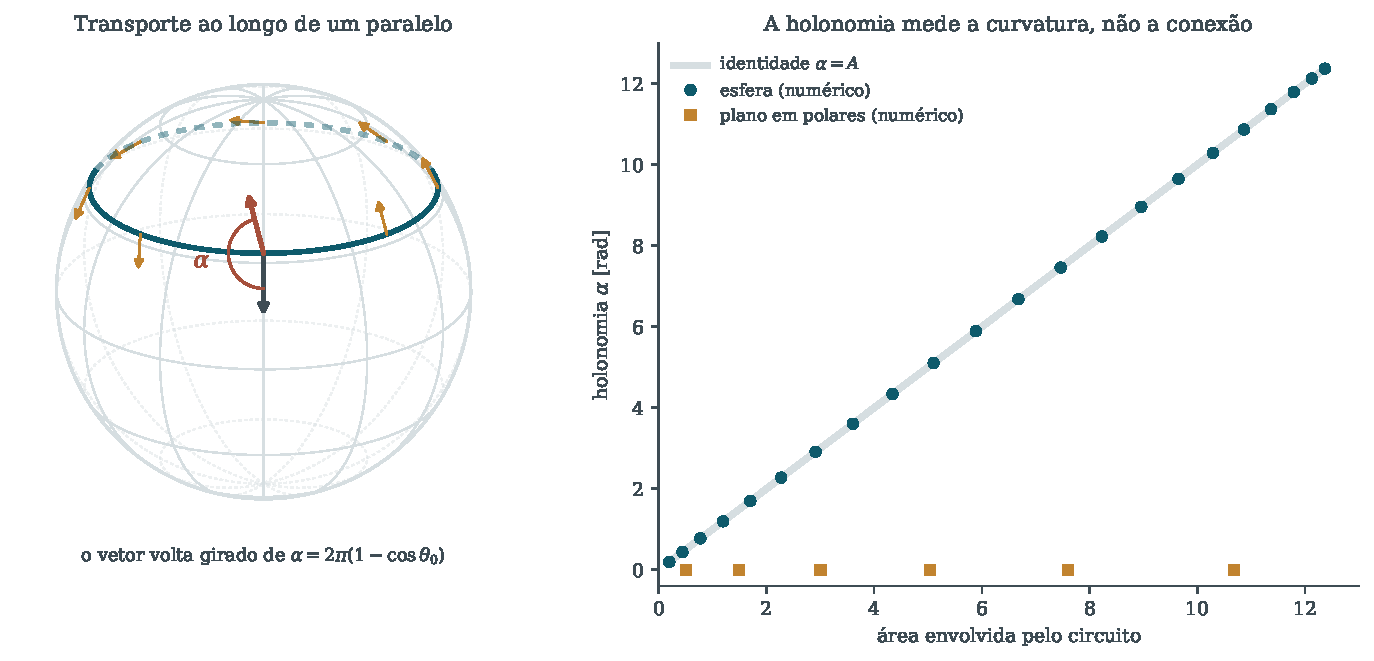
\includegraphics[width=\linewidth]{figuras/cap07_holonomia.pdf}
  \caption{À esquerda, o vetor transportado ao longo de um paralelo da
  esfera: ele gira continuamente e não retorna à direção inicial. À direita,
  a holonomia medida contra a área envolvida pelo circuito. Os pontos da
  esfera caem sobre a reta $\alpha=A$ --- a curvatura de Gauss é $1$ e a
  holonomia \emph{é} a área. Os quadrados são o plano euclidiano em
  coordenadas polares: símbolos de Christoffel não nulos, holonomia nula
  para qualquer circuito.}
  \label{fig:cap07-holonomia}
\end{figure}

\subsubsection*{Riemann por diferenças finitas}

Nada no cálculo de $\Gamma$ e de $R^a{}_{bcd}$ exige álgebra simbólica: são
derivadas da métrica. Basta implementá-las com diferenças centrais e a
máquina serve para qualquer métrica dada como função.

\begin{saida}
\begin{lstlisting}[style=rgsaida]
   esfera unitaria        R = +2.00000000   (exato: +2.0)
   plano em polares       R = +0.00000001   (exato: +0.0)
   Schwarzschild em r = 8 M:
      max |R_munu|  = 9.419e-07   (exato: 0)
      R             = -9.647e-09          (exato: 0)
      Kretschmann   = 0.0001831053
      48 M^2/r^6    = 0.0001831055
      componentes nao nulas de R_abcd: 24 de 256
      independentes sob as simetrias:  6   (o maximo em 4D e' 20)
\end{lstlisting}
\end{saida}

Três leituras. A primeira: o Ricci de Schwarzschild dá $10^{-7}$ em vez de
zero, e isso é o piso de precisão das diferenças finitas, não física --- a
métrica \emph{é} solução exata de vácuo. A segunda: o escalar de Kretschmann
reproduz $48M^2/r^6$ em sete dígitos, mostrando que o Riemann completo é bem
diferente de zero embora sua contração seja nula. É essa distinção que
permite maré e onda gravitacional no vácuo.

A terceira é a mais instrutiva. Das $256$ componentes de $R_{abcd}$, apenas
$24$ são não nulas em Schwarzschild, e as simetrias as reduzem a $6$
independentes --- bem abaixo das $20$ que uma métrica genérica em quatro
dimensões teria. Simetria esférica e estaticidade não são hipóteses de
conveniência: elas cortam o problema por um fator maior que três.

\subsubsection*{Desvio geodésico}

Em duas dimensões o tensor de Riemann tem uma única componente independente,
e ela é a curvatura de Gauss. A equação de desvio geodésico se reduz a
\begin{equation}
  \rd{^2\xi}{s^2}+K(s)\,\xi=0,
  \label{eq:cap07-desvio}
\end{equation}
com $\xi$ a separação própria entre duas geodésicas vizinhas. O teste é
honesto: $K$ é lido do tensor de Riemann numérico, ponto a ponto, e
\eqref{eq:cap07-desvio} é integrada sem nunca usar a forma fechada da
métrica.

\begin{saida}
\begin{lstlisting}[style=rgsaida]
  K exato    K medido      s    xi integrado    xi analitico   erro rel.
        1    1.000000   0.50    0.0095885108    0.0095885108    9.80e-10
        1    1.000000   1.50    0.0199498998    0.0199498997    4.15e-09
        1    1.000000   2.40    0.0135092639    0.0135092636    2.14e-08
        0    0.000000   0.50    0.0100000000    0.0100000000    2.56e-11
        0    0.000000   1.50    0.0300000000    0.0300000000    1.86e-10
        0    0.000000   2.40    0.0480000000    0.0480000000    7.16e-10
       -1   -1.000000   0.50    0.0104219061    0.0104219061    2.04e-09
       -1   -1.000000   1.50    0.0425855894    0.0425855891    5.96e-09
       -1   -1.000000   2.40    0.1093245855    0.1093245843    1.11e-08
\end{lstlisting}
\end{saida}

\begin{figure}[htbp]
  \centering
  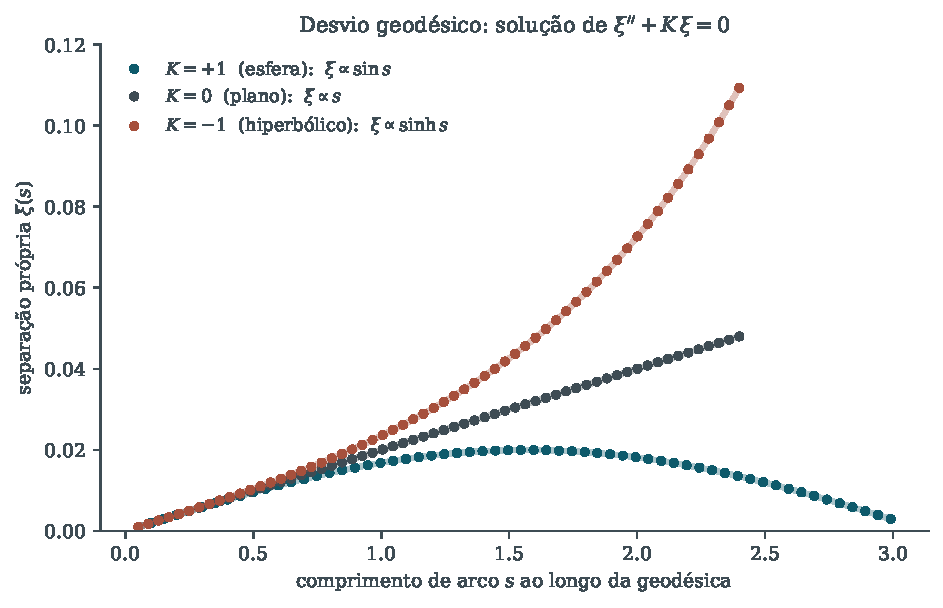
\includegraphics[width=0.82\linewidth]{figuras/cap07_desvio_geodesico.pdf}
  \caption{Separação própria entre duas geodésicas que partem do mesmo ponto,
  para curvatura constante positiva, nula e negativa. Os pontos são a
  integração de~\eqref{eq:cap07-desvio} com $K$ extraído do Riemann numérico;
  as faixas claras são $\sin s$, $s$ e $\sinh s$. Na esfera a separação passa
  por um máximo e volta a zero em $s=\pi$: as geodésicas se reencontram no
  ponto antípoda. No plano ela cresce linearmente para sempre. No espaço
  hiperbólico, exponencialmente.}
  \label{fig:cap07-desvio}
\end{figure}

\begin{central}
Compare a primeira linha com a última. Em $s=2{,}4$, duas geodésicas que
partiram com a mesma separação inicial estão a $0{,}0135$ na esfera e a
$0{,}109$ no espaço hiperbólico --- oito vezes mais longe. Nenhuma força atua
em nenhum dos dois casos: as curvas são geodésicas, o movimento é livre. A
diferença inteira está no sinal de um número lido da métrica. É esta a
afirmação que, transposta para quatro dimensões e para $R^\mu{}_{\alpha\nu\beta}
U^\alpha\xi^\nu U^\beta$, vira o efeito de maré --- e vira, no
Capítulo~\ref{cap:ondas}, o anel de partículas deformado por uma onda.
\end{central}

\subsection{Mathematica}

\programa[Simetrias do Riemann, contagem de componentes e a divergência do tensor de Einstein. Define as rotinas reaproveitadas nos capítulos seguintes.]{codigo/cap07\_curvatura\_simbolico.wl}

O simbólico faz aqui o que o numérico não consegue: provar as simetrias em
vez de conferi-las num ponto. O script define as rotinas
\texttt{Christoffel}, \texttt{Riemann} e \texttt{Ricci} usadas também nos
Capítulos \ref{cap:ondas}, \ref{cap:schwarzschild} e seguintes, e verifica as
quatro simetrias de $R_{abcd}$ de uma vez.

A contagem que essas simetrias produzem é $n^2(n^2-1)/12$:

\begin{center}
\small
\begin{tabular}{ccccp{5.4cm}}
\toprule
$n$ & Riemann & Ricci & Weyl & consequência \\
\midrule
2 & 1 & 1 & 0 & uma só componente: a curvatura de Gauss \\
3 & 6 & 6 & 0 & Ricci determina Riemann; não há ondas gravitacionais \\
4 & 20 & 10 & 10 & sobra o tensor de Weyl: maré e radiação no vácuo \\
5 & 50 & 15 & 35 & \\
\bottomrule
\end{tabular}
\end{center}

A linha $n=3$ merece atenção. Em $2+1$ dimensões, $R_{\mu\nu}=0$ implica
$R^\rho{}_{\sigma\mu\nu}=0$: o vácuo é rigorosamente plano e a gravidade não
tem graus de liberdade propagantes. Só a partir de quatro dimensões o tensor
de Weyl abre espaço para geometria dinâmica em regiões sem matéria.

O último bloco do script verifica a identidade de que tudo depende. Ele
constrói $G_{\mu\nu}$ para a métrica esfericamente simétrica mais geral
possível, com $A(r)$ e $B(r)$ deixadas como funções livres, e toma sua
divergência covariante --- que resulta identicamente nula.

\begin{central}
A divergência covariante do tensor de Einstein se anula para uma métrica
esfericamente simétrica \emph{qualquer}, com $A(r)$ e $B(r)$ funções livres.
Nenhuma equação de campo foi imposta. Isso deixa claro o que
$\nabla_\mu G^{\mu\nu}=0$ realmente é: não uma propriedade das soluções, mas
um teorema de geometria diferencial, válido para toda métrica. É por isso que
ele pode ser usado como \emph{argumento} para escolher $G_{\mu\nu}$ como lado
geométrico das equações de campo, em vez de ser uma consequência delas.
\end{central}

